%%
%
% ARQUIVO: cap-02.tex
%
% VERSÃO: 1.0
% DATA: Maio de 2017
% AUTOR: Carla Cosenza, Matheus Mello, Rebeca Reis
% 
%  Arquivo tex de exemplo de capítulo do documento de Projeto de Fim de Curso.
%
% ---
% DETALHES
%  a. todo capítulo deve começar com \chapter{•}
%  b. usar comando \noindent logo após \chapter{•}
%  c. citações para referências podem ser
%       i. \citet{•} para citações diretas (p. ex. 'Segundo Autor (2015)...'
%       ii. \citep{•} para citações indiretas (p. ex. '... (AUTOR, 2015)...'
%  d. notas de rodapé devem usar dois comandos
%       i. \footnotemark para indicar a marca da nota no texto
%       ii. \footnotetext{•}, na sequência, para indicar o texto da nota de rodapé
%  e. figuras devem seguir o exemplo
%       i. devem ficar no diretório /img e devem ser no formato EPS
%  f. tabelas devem seguir o exemplo
%  g. figuras e tabelas podem ser colocadas em orientação landscape
%       i. figuras: usar \begin{sidewaysfigure} ... \end{sidewaysfigure}
%                   em vez de \begin{figure} ... \end{figure}
%       ii. tabelas: usar \begin{sidewaystable} ... \end{sidewaystable}
%                    em vez de \begin{table} ... \end{table}
%  h. toda figura e tabela deve ser referenciada ao longo do texto com \ref{•}
% ---
%%

\chapter{Implementação e avaliação}
\noindent

\section{Processo de teste das features implementadas}

As partes referidas ao analisador léxico e sintático são relativamente fáceis de testar. Na main do projeto existem flags para acionar apenas partes específicas do compilador (tal como o gcc e o clang tem essas opções, por exemplo).

Cada suíte de teste tem uma pasta para si. A pasta leva o nome da suíte de teste. Cada suíte de teste é composta por n casos de teste (compostos de um teste.ha e  um teste.answer, onde o .ha representa o input para o compilador e o .answer o resultado produzido esperado) e um script shell script.sh. 

O script é responsável por acionar o compilador com os parâmetros corretos; testar cada um dos casos; comparar a resposta produzida com a resposta esperada e contabilizar o número de testes bem-sucedidos e mal-sucedidos. A diferença entre as respostas é calculada pelo comando diff do Unix e permite verificar exatamente quais são as linhas em que a diferença ocorre.

Ter um script.sh para cada suíte de teste é uma abstração que permite casos de teste mais elaborados: desde testar se o compilador reage a um input incorreto com a mensagem de erro apropriada a compilar e executar inputs fornecidos verificando se a execução está nos conformes.

Finalmente, cada suíte de teste tem uma regra no makefile para facilitar o seu uso. O padrão de nome é test<nome da suíte de teste>. Para executar a suíte de teste lexical, basta digitarmos make testlexical.

Há ainda, uma regra no makefile nomeada test. Ela possui como dependências todas as regras de teste. Com ela, é possível executar todos os testes do projeto simplesmente digitando 'make test' pela linha de comando no diretório raiz do projeto (veja figura \ref{erro}).

\begin{figure}[h]
    \centering
	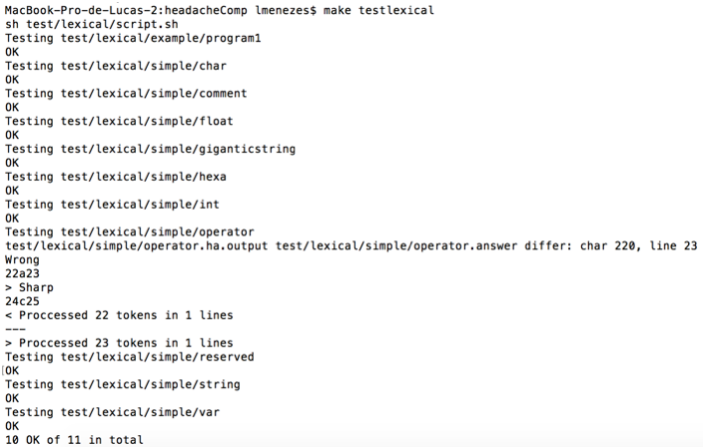
\includegraphics[]{TD/img/erro.png}
	\caption{Exemplo de erro em um arquivo de teste}
	\label{erro}
\end{figure}

\section{Método de debug ou modo run}

Há ainda o método utilizado para depurar a geração de código propriamente dita. Nos arquivos fonte, há um interpretador brainfuck (bfi) utilizado para auxiliar o desenvolvimento. 

Ele é habilitado na main por uma flag, tal como outras opções do compilador. É executado após a compilação e permite ao hac verificar o estado da memória do interpretador após (e, possivelmente, durante) a execução do programa. Isso é especialmente útil para depurar a implementação de variáveis, parâmetros e operações nos seus estados iniciais de desenvolvimento.

Esse modo conta com uma função que busca valores preenchidos na memória do interpretador. Ela é usada para decidir a partir de qual célula o conteúdo da memória será mostrado. 

Apesar desse modo ter sido implementado apenas para fins de debug, ele pode se tornar uma feature do compilador hac. Muitas linguagens de programação permitem, no seu compilador, um modo compile e um modo run.

\begin{verbatim}
    if(!noDebug)
    {
        printf("Debugging\n");
        char* program = readFile(bf_name);
        printf("exec\n");
        int used = execute(program, 30000, 1);
        free(program);
        printf("printing memory\n");
        printAllWrittenMemory();
        printf("used %d cells (bytes) to run\n", used);
    }
    
    Debugging
    exec
    144
    11
    222
    1
    printing memory
    start 0: |0|0|0|0|0|0|144|11|222|1|0|0|0|2|11|0|30|33|
    start 18: |0|64|0|0|1|0|0|0|0|0|0|0|0|0|0|0|
    used 36 cells (bytes) to run
\end{verbatim}

Apesar desse modo ter sido implementado apenas para fins de debug, ele pode se tornar uma feature do compilador hac. Muitas linguagens de programação permitem, no seu compilador, um modo compile e um modo run.

Alguns exemplos de programas que o hac pode transformar em brainfuck:

\begin{verbatim}
------ example.ha -------
void main() {
	@"Hello World!\n";
}
----- sub.ha -----
void main() {
	byte a;
	byte b;
	byte c;
	a = 3-1+7; 
	b = a-10;
	c = 21;
	c = c - 256;
-------divide.ha -------
void main(){
	byte a;
	byte b;
	byte c;
	byte d;
	a = (10*6+3)/7; /* 63/7 = 9 */
	b = (10*23-5*23)/23; /* 5*23/23 = 5 */
	c = 0/0+10/10; /* 0/0 converts to zero in headache */
	d = a/a + b/b + c/c;
	@"a: "; @a; @"\n";
	@"b: "; @b; @"\n";
	@"c: "; @c; @"\n";
	@"d: "; @d; @"\n";
}


-------conditions.ha ------- 
void main() {
	byte a;
	a = 10;
	if(a>1) { 
		if(a>2){ 
			if(a>3) { 
				if(a>4){ 
					if(a>5){ 
						@a;@" is greater than five\n";
					}
					@a;@" is greater than four\n";
				}
				@a;@" is greater than three\n";
			}
			@a;@" is greater than two\n";
		} 
		@a;@" is greater than one\n";

	} else if(true) {
		@"Block 1";@"\n";
	} else if(2==2) {
		@"Block 2";@"\n";
	} else if(3<4) {
		@"Block 3";@"\n";
	}
}

-------count.ha -------
void main()
{
	byte a;
	a=1;
	while(a){
		@a;@"\n";
		a++;
	}
}
-------while2.ha -------
void main(){
	byte i,j;
	byte x,y,r;
	i = 2;
	r = 0;
	while(i){
		j=2;
		while(j){
			//@"y ";
			j--;
			r++;
		}
		i--;
		//@"x\n";
	}
	@"Result is "; @r; @"\n";
}




-------power.ha -------
short pow(short x, short y){
	short r,z;
	r=1;
	z = y;
	while(z){
		r = r*x;
		z--;
	}
	return r;
}
void main(){
	short a,b;
	a=2;
	b=10;
	@"pow(";@a;@",";@b;@") = ";
	@pow(a,b);@"\n";
}

\end{verbatim}

\section{Comentários sobre implementação}

Para fazer com que a main() executasse, ela é a única função cuja definição é compilada (forçando um call).

FIGURA/CODIGO

A existência desse tipo de exceção me leva a crer que não existe nenhuma boa razão para não incluir um modo interativo em Headache tal qual linguagens como Lua e Python. É muito provável que a estrutura do código ficasse até mais fluída.

\section{Comentários sobre defeitos}

Dentre os problemas encontrados temos:

\begin{itemize}
    \item Organização de código no codegen.c: Módulo muito grande que além de conter código desnecessário é pouco modularizado. Sugestão: Separar as funções que implementam os algoritmos da Brainfuck Algorithms da transformação da AST em código output. Status: Não implementado.
    \item Corrupção de registradores por condições em loops while. Solução proposta: adicionar registradores ou compilar todas as variáveis e temporários para endereços estáticos em tempo de compilação. Status: Não implementado completamente. Há bugs.
    \item Combinar a geração de código para tipos byte e short de forma nativa não foi feito. Ao invés, foi adotada uma solução alternativa: detectar se o programa usa shorts e ativar uma flag; Compilá-lo usando apenas variáveis bytes e expandir o programa todo ao final. Isso gera uma semântica diferente (algumas variáveis em short contra todas em short), porém permite, em versão beta, a feature de shorts em brainfuck
\end{itemize}

\section{Features pensadas porém não implementadas}

\begin{itemize}
    \item tipo bit
\end{itemize}

Ter um tipo próprio para operações booleanas, um tipo que só pudesse assumir os valores 0 e 1 e que essa propriedade fosse checada estaticamente (em tempo de compilação). Se não faz diferença nos registradores usuais das CPUs essa diferença, em brainfuck certamente faz (menos incrementos e decrementos, algoritmos de checagem mais rápidos). Esse tipo seria conveniente denominado bit (para fazer par ao tipo byte)

\begin{itemize}
    \item tipo float/real
\end{itemize}

Implementar o tipo real/float baseando-se na implementação antiga do tipo real em pascal, (quando ainda não era implementado em hardware, mas utilizando libs de algortimos de manipulação de bits). Foi cortado do projeto devido a estar claramente fora do escopo do tempo.

\begin{itemize}
    \item inline brainfuck
\end{itemize}

Permitir que o programador, ao escrever código Headache, tivesse alguma estrutura que o permitisse otimizar um processamento com o seu próprio código brainfuck.

\begin{itemize}
    \item ibs e include
\end{itemize}

Permitir a inclusão de libs com funções comuns como print(), println(), pow(x,y), sqrt(x). 

O programador Headache escreveria no topo do documento algo como "include stdprint" para utilizar a println(). Escreveria algo como “include stdmath” para utilizar a pow() e a sqrt(). Poderia incluir o tipo real/float  com algo como include “stdreal”.

Headache podia ter um diretório Headers/ com o código em Headache dessas libs (stdprint.ha, stdmath.ha), que seria, por baixo dos panos, colado no topo do documento e compilaria normalmente.

\begin{itemize}
    \item for
\end{itemize}

for ao estilo C como açúcar sintático para o while foi planejado. Porém devido a dificuldades de implementação, ele é representado de uma forma diferente na AST e sua geração de código é independente. \newline


Como se pode observar, muitas dessas features que não chegaram a ser incluídas seriam utilizadas juntas, ou uma ajudaria a implementar a outra.
